\section{The Discrete Ordinates Method}
\label{sec:SN}

The discrete ordinates method is an approach for discretization of the angular dependence of \(\psi\); the angular variable is allowed to obtain a discrete set of values (ordinates) such that the angular flux corresponding to each discrete direction \(\hO_n\) is:

\beq
\psi_n(\vv{r},E,t)\equiv\psi(\vv{r},E,\hO_n,t)
\eeq

for \(n=1,\cdots,N\). The \gls{nte} can then be written for each discrete direction \(\hO_n\) by approximating the scattering and fission angular integrals using a quadrature rule with quadrature points set equal to the angular ordinates:

\beqa
\frac{\partial}{\partial t}\left(\frac{\psi_n(\vv{r},E,t)}{v(E)}\right)+\hO_n\cdot\nabla\psi_n(\vv{r},E,t)+\Sigma_{t,n}(\vv{r},E,t)\psi_n(\vv{r},E,t)=\hspace{3cm}\\
\sum_{n'=1}^Nw_{n'}\dEprime \Sigma_s(\vv{r},E'\rightarrow E',\hO_{n'}\rightarrow\hO_n,t)\psi_{n'}(\vv{r},E',t)+\hspace{2cm}\\
\chi_{p,n}(E)\left(1-\beta\right)\sum_{n'=1}^Nw_{n'}\dEprime\nu(E')\Sigma_{f,n
'}(\vv{r},E',t)\psi_n(\vv{r},E,t)+\hspace{1cm}\\
\sum_{j=1}^J\chi_{d,j,n}(E)\lambda_jC_j(\vv{r},t)+S_n(\vv{r},E,t)
\eeqa

This discrete ordinates method is often referred to as the ``S$_{\text{N}}$'' method. The S$_{\text{N}}$ method is named after the early one-dimensional treatments that used the trapezoidal quadrature set, which is equivalent to treating the angular dependence as \(N\) straight line segments. The S$_{\text{N}}$  method is the primary way in which the transport equation is discretized in angle, since it 1)~has a simple derivation, 2)~closely resembles the Boltzmann transport equation, and 3)~does not have to deal with as many strange math properties as the P$_{\text{N}}$  method described in Section \ref{sec:PN}. In 1-D, S$_{\text{N}}$  is equivalent to Legendre expansions of the angular dependence.

To begin, the scattering and external source are expanded into spherical harmonics. Assuming azimuthal symmetry, the scattering cross section can be expanded as in Eq. \eqref{eq:ScatteringLegendre2}. Beginning with the fixed-source problem in Eq. \eqref{eq:TE_fixedsource}, repeated here for reference:

\begin{equation*}
\begin{aligned}
 \hO  \cdot\nabla\psi(\vv{r}, E, \hO  ) + 
 \Sigma_t(\vv{r},E)\psi(\vv{r}, E, \hO  ) = \\
S(\vv{r}, E, \hO  ) + \int_{0}^{\infty}dE' \int_{4\pi}^{ } d\hO  ' \Sigma_s(\vv{r}, E'\rightarrow E, \hO  '\rightarrow\hO  )\psi(\vv{r}, E', \hO  ')\\
\end{aligned}
\end{equation*}

The scattering source is expanded in Legendre polynomials according to Eq. \eqref{eq:ScatteringLegendre2}.

\begin{equation}
\begin{aligned}
 \hO  \cdot\nabla\psi(\vv{r}, E, \hO  ) + 
 \Sigma_t(\vv{r},E)\psi(\vv{r}, E, \hO  ) = \\
S(\vv{r}, E, \hO  ) + \int_{0}^{\infty}dE' \int_{4\pi}^{ } d\hO  ' \sum_{l=0}^{\infty}\frac{2l+1}{4\pi}\Sigma_{s,l}(\vv{r}, E'\rightarrow E)P_l(\hO  \cdot\hO  ')\psi(\vv{r}, E', \hO  ')\\
\end{aligned}
\end{equation}

Because the scattering operator is real (i.e. not complex), \(P_l(\hO  \cdot\hO  ')\) can be expanded in real and complex components, and then the complex components set to zero. The end result of this expansion, where only real components result, is given in Eq. \eqref{eq:FullExpansion5}. Using this expansion, the scattering term becomes:

\begin{equation}
\label{eq:ScatteringSourceSN}
\begin{aligned}
\int_{0}^{\infty}dE' \int_{4\pi}^{ } d\hO  ' \sum_{l=0}^{\infty}\Sigma_{s,l}(\vv{r}, E'\rightarrow E)\left\lbrack Y_{l0}^e(\hO  )Y_{l0}^e(\hO  ')+\sum_{m=1}^{l}\left(Y_{lm}^e(\hO  )Y_{lm}^{e}(\hO  ')+Y_{lm}^o(\hO  )Y_{lm}^{o}(\hO  ')\right)\right\rbrack\psi(\vv{r}, E', \hO  ')\\
\end{aligned}
\end{equation}

\begin{tcolorbox}[breakable]
For simplicity, Eq. \eqref{eq:ScatteringSourceSN} is sometimes written in compact notation by defining:

\begin{equation}
\label{eq:FluxMoments31}
\begin{aligned}
e_{lm}(\vv{r},E')=\int_{4\pi}^{}d\hO  'Y_{lm}^e(\hO  ')\psi(\vv{r}, E',\hO  ')\\
o_{lm}(\vv{r},E')=\int_{4\pi}^{}d\hO  'Y_{lm}^o(\hO  ')\psi(\vv{r}, E',\hO  ')\\
\end{aligned}
\end{equation}

Inserting these definitions removes, in compact notation, the angular dependency on \(\hO  '\):

\begin{equation}
\label{eq:ScatteringSourceSNSimple}
\begin{aligned}
\int_{0}^{\infty}dE' \sum_{l=0}^{\infty}\Sigma_{s,l}(\vv{r}, E'\rightarrow E)\left\lbrack Y_{l0}^e(\hO  )e_{l0}(\vv{r},E')+\sum_{m=1}^{l}\left(Y_{lm}^e(\hO  )e_{lm}(\vv{r},E')+Y_{lm}^o(\hO  )o_{lm}(\vv{r},E')\right)\right\rbrack\\
\end{aligned}
\end{equation}
\end{tcolorbox}

The order of the scattering expansion in Eq. \eqref{eq:ScatteringSourceSN} is infinite because \(0\leq l\leq\infty\). However, this expansion must be truncated, and hence \(N\) in \(0\leq l\leq N\) represents the order of the scattering expansion. This order is referenced sometimes as the ``\(P_N\) scattering expansion.'' 

Likewise, the external source can also be expanded into real and imaginary components, and the imaginary components set to zero. The only differences are that there is no cross section moment present (since an external source does not depend on any cross section of the medium) and the source is not proportional to the angular flux. Hence, the external source is:

\begin{equation}
\label{eq:14}
S(\vv{r},E, \hO  )=\int_{4\pi}^{}d\hO  '\sum_{l=0}^{\infty}S(\vv{r},E', \hO  ')\left\lbrack Y_{l0}^e(\hO  )Y_{l0}^e(\hO  ')+\sum_{m=1}^{l}\left(Y_{lm}^e(\hO  )Y_{lm}^{e}(\hO  ')+Y_{lm}^o(\hO  )Y_{lm}^{o}(\hO  ')\right)\right\rbrack 
\end{equation}

\begin{tcolorbox}[breakable]
For simplicity, Eq. \eqref{eq:14} is sometimes written in compact notation by defining:

\begin{equation}
\begin{aligned}
s_{lm}(\vv{r},E')=\int_{4\pi}^{}d\hO  'Y_{lm}^e(\hO  ')S(\vv{r}, E',\hO  ')\\
v_{lm}(\vv{r},E')=\int_{4\pi}^{}d\hO  'Y_{lm}^o(\hO  ')S(\vv{r}, E',\hO  ')\\
\end{aligned}
\end{equation}

Inserting these definitions removes, in compact notation, the angular dependency on \(\hO  '\):

\begin{equation}
\label{eq:ExternalSourceSNSimple}
\begin{aligned}
S(\vv{r},E, \hO  )=\sum_{l=0}^{\infty}\left\lbrack Y_{l0}^e(\hO  )s_{l0}(\vv{r},E)+\sum_{m=1}^{l}\left(Y_{lm}^e(\hO  )s_{lm}(\vv{e},E)+Y_{lm}^o(\hO  )v_{lm}(\vv{r},E)\right)\right\rbrack
\end{aligned}
\end{equation}
\end{tcolorbox}

The external source expansion in Eq. \eqref{eq:ExternalSourceSNSimple}, and the scattering source expansion in Eq. \eqref{eq:ScatteringSourceSNSimple}, are then combined in the neutron transport equation to give the \(S_N\) equations:

\begin{equation}
\label{eq:SnGeneral}
\begin{aligned}
 \hO  \cdot\nabla\psi(\vv{r}, E, \hO  ) + 
 \Sigma_t(\vv{r},E)\psi(\vv{r}, E, \hO  ) = \\
\sum_{l=0}^{N}\left\lbrack Y_{l0}^e(\hO  )s_{l0}(\vv{r},E)+\sum_{m=1}^{l}\left(Y_{lm}^e(\hO  )s_{lm}(\vv{e},E)+Y_{lm}^o(\hO  )v_{lm}(\vv{r},E)\right)\right\rbrack+\\
\int_{0}^{\infty}dE' \sum_{l=0}^{N}\Sigma_{s,l}(\vv{r}, E'\rightarrow E)\left\lbrack Y_{l0}^e(\hO  )e_{l0}(\vv{r},E')+\sum_{m=1}^{l}\left(Y_{lm}^e(\hO  )e_{lm}(\vv{r},E')+Y_{lm}^o(\hO  )o_{lm}(\vv{r},E')\right)\right\rbrack\quad\\
\end{aligned}
\end{equation}

where the infinite sums in \(l\) have been truncated to \(N\) terms. For \(N\), \((N+1)^2\) moments must be computed. 
We replace each occurrence of \(\hO  \) in Eq. \eqref{eq:SnGeneral} by \(\hO  _a\) to indicate a particular direction. Then, Eq. \eqref{eq:SnGeneral} applies for each direction. All other terms in the equation are then integrated using quadrature rules. 

\begin{equation}
\label{eq:SnGeneral}
\begin{aligned}
 \hO  _a\cdot\nabla\psi_a(\vv{r}, E) + 
 \Sigma_t(\vv{r},E)\psi_a(\vv{r}, E) = \\
\sum_{l=0}^{N}\left\lbrack Y_{l0}^e(\hO  _a)s_{l0}(\vv{r},E)+\sum_{m=1}^{l}\left(Y_{lm}^e(\hO  _a)s_{lm}(\vv{e},E)+Y_{lm}^o(\hO  _a)v_{lm}(\vv{r},E)\right)\right\rbrack+\\
\int_{0}^{\infty}dE' \sum_{l=0}^{N}\Sigma_{s,l}(\vv{r}, E'\rightarrow E)\left\lbrack Y_{l0}^e(\hO  _a)e_{l0}(\vv{r},E')+\sum_{m=1}^{l}\left(Y_{lm}^e(\hO  _a)e_{lm}(\vv{r},E')+Y_{lm}^o(\hO  _a)o_{lm}(\vv{r},E')\right)\right\rbrack\quad\\
\end{aligned}
\end{equation}

where notation has been simplified by indicating that \(\psi_a(\vv{r},E)\equiv\psi(\vv{r},E,\hO  _a\). In addition, all the moments are computed using the quadrature rule:

\begin{equation}
e_{lm}=\sum_{n=1}^{N} w_nY_{lm}^e(\hO  _n)\psi_a(\vv{r},E)
\end{equation}

and so forth for the remaining moments. Note that the quadrature rule used is a quadrature rule in angle. It is customary to select the quadrature points in this quadrature rule, i.e. the \(\hO  _n\) in the above equation, to match the discrete choices of \(\hO  _a\) that appear in the \(S_N\) equations. 

The order of the \(S_N\) method and the order of the \(P_L\) expansion discussed in reference to Eq. \ref{eq:ScatteringMomentsLegendre} result in different numbers of discrete directions and angular moments depending on the dimensionality of the problem. In 1-D, there are \(N\) discrete directions and \(L\) angular moments. In 2-D however, there are \(N(N+2)/2\) directions and \((L+1)(L+2)/2\) angular moments, and in 3-D, there are \(N(N+2)\) directions and \((L+1)^2\) moments. 

The \(S_N\) method will converge to the true solution provided the quadrature rule accurately integrates the spherical harmonics. An important phenomena that sometimes arises with the \(S_N\) method is ray effects. Because we constrain the flux to travel only along discrete directions, nothing can be said about the accuracy not along those angles. Non-physical ``crown-like'' patterns can result, but this can be fixed by computing a first-collided source as the actual source to be used in the computation, providing a diffuse starting source without significantly reducing accuracy. 

\subsection{Quadrature}

This section describes the various quadrature sets typically used with the discrete ordinates method. The level-symmetric quadrature set described in Section \ref{sec:LevelSymmetric} is the quadrature set most often associated with the discrete ordinates method. The quadrature set must be normalized such that integration over the unit sphere of a constant equals \(4\pi\):

\begin{equation}
\label{eq:QuadratureNormalization}
\int_{4\pi}^{}d\hO  =\sum_{n=1}^{N} w_n =4\pi
\end{equation}

Quadrature sets may be symmetric or non-symmetric, a construction that may be useful if streaming is expected to occur preferentially in some directions.

\subsubsection{Level-Symmetric Quadrature}
\label{sec:LevelSymmetric}
The level-symmetric quadrature set uses \(N(N+2)\) symmetric angular directions per spatial location. Due to the symmetry constraint, not all of the choices for the quadrature points are independent; there is only one degree of freedom for each choice of quadrature set. A second constraint given by Eq. \eqref{eq:QuadratureNormalization} then narrows down the options for the quadrature set. With these two constraints, the S$_2$ quadrature is fixed, but several options remain for higher order sets. 

\subsubsubsection{LQ$_{\text{N}}$ Quadrature}

With the same symmetry and normalization constraints as the level-symmetric quadrature set described in Section \ref{sec:LevelSymmetric}, the LQ$_{\text{N}}$ set imposes the additional requirement that the quadrature should correctly integrate as many Legendre polynomials as possible. 

\subsubsection{Spatial Discretization}

The \(S_N\) equations provide the framework to discretize the angular flux in angle, but the equations still must be discretized in space. In general, there are two different means to perform spatial discretization - cell balance methods, which preserve conservation of the solution, and finite element methods, which do not necessarily preserve conservation of the solution. In a single mesh cell, cell balance methods will provide a statement that is equivalent to conservation of neutrons, while finite element methods satisfy the governing equation in a weighted-integral sense. For simplicity, all of the spatial discretization schemes discussed here are applied to the simplified transport equation that neglects time dependence and assumes some angular discretization has already been applied to \(\psi\) such that it is independent of angle (in each of these equations):

\begin{equation}
\label{eq:SimpleTE}
\hO  \cdot\nabla\psi(\vv{r},E)+\Sigma_t{\vv{r},E}\psi(\vv{r},E)=S(\vv{r},E)
\end{equation}

where \(S\) represents the scattering, fission, and external sources. There will be one of these equations for each discrete direction in the \(S_N\) method. For all the following discretization schemes, a Cartesian mesh given in Fig. \ref{fig:CartesianDiscretization} is assumed, with \(i\) representing indices in the \(x\)-direction, \(j\) in the \(y\)-direction, and \(k\) in the \(z\)-direction.

\begin{figure}[H]
\centering
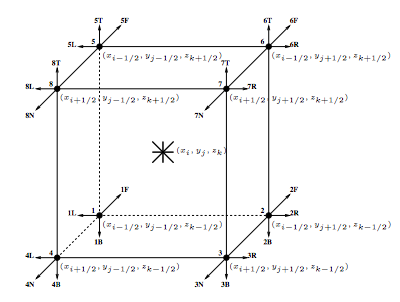
\includegraphics[width=0.6\linewidth]{figures/CartesianDiscretization.jpg}
\caption{Cartesian discretization to be used for the cell balance schemes.}
\label{fig:CartesianDiscretization}
\end{figure}

